\tikzset{button/.style={
% First preaction: Fuzzy shadow
preaction={fill=black,path fading=circle with fuzzy edge 20 percent,
opacity=.5,transform canvas={xshift=1mm,yshift=-1mm}},
% Second preaction: Background pattern
preaction={pattern=#1,
path fading=circle with fuzzy edge 15 percent},
% Third preaction: Make background shiny
preaction={top color=white,
bottom color=black!50,
shading angle=45,
path fading=circle with fuzzy edge 15 percent,
opacity=0.2},
% Fourth preaction: Make edge especially shiny
preaction={path fading=fuzzy ring 15 percent,
top color=black!5,
bottom color=black!80,
shading angle=45},
inner sep=2ex
},
button/.default=horizontal lines light blue,
circle}
      \tikzstyle{bordered} = [draw,outer sep=0,inner sep=1,minimum size=10]
    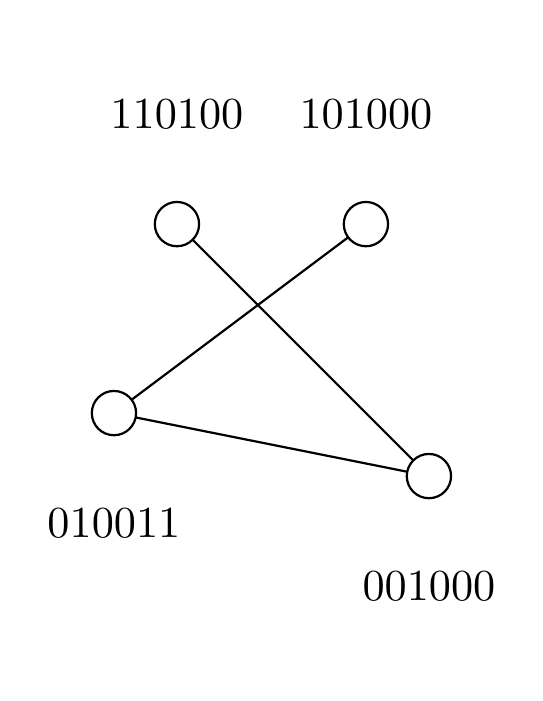
\begin{tikzpicture}[thick,scale=1.6, every node/.style={scale=1.6}]

\node [draw,outer sep=0,inner sep=1,minimum size=10, label = 110100] (v1) at (-1.5,2) {};
\node [draw,outer sep=0,inner sep=1,minimum size=10, label = 101000] (v3) at (0,2) {};
\node [draw,outer sep=0,inner sep=1,minimum size=10, label = below: 010011] (v4) at (-2,0.5) {};
\node [draw,outer sep=0,inner sep=1,minimum size=10, label = below: 001000] (v2) at (0.5,0) {};
\draw  (v1) edge (v2);
\draw  (v3) edge (v4);
\draw  (v4) edge (v2);
\end{tikzpicture}